\documentclass{article}
\usepackage[utf8]{inputenc} % - Defines what coding LaTeX uses. Use this one.
\usepackage{graphicx} % - Package for including images in the document.
\usepackage{amsmath}
\usepackage{mathtools}
\usepackage{gensymb}
\usepackage{float}
\usepackage{subfiles}
\usepackage{array}
\usepackage{tikz}
\usepackage{tikz-timing}
\usepackage{pgf-umlsd}
\usepackage[backend=biber]{biblatex}
\addbibresource{refs.bib}
\graphicspath{ {pictures/} } % - Path to where the images are located on your computer. In this case I have a folder (look to the left) "Images" where the images are gathered.


%%%%%%%%%%%%%%%%%%%%%%%%%%%%%%%%%%%%%%%%%%%%%%%%%%%%%%%%%%%%%%
% -               Title and affiliation                    - %
%%%%%%%%%%%%%%%%%%%%%%%%%%%%%%%%%%%%%%%%%%%%%%%%%%%%%%%%%%%%%%

\title{}

\author{}


\date{\today}

\begin{document}

\section{Theory}
Theory behind the design Arrowhead, SoS etc

\section{Problem formulation}
\label{sec:software:problem_formulation}

The problem solved by the software is to create a system according to the following high level functional requirements:\\
\begin{enumerate}
    \item A user can construct a mission for the robot to do some meaningful work.
    \item The mission can be sent to the robot and be executed in a way so the work is done.
    \item A higher priority mission can preempt a lower priority mission.
    \item Have a distributed, flexible and fault tolerant system.
\end{enumerate}

\section{Methods}

% software requirements.
% Design goals.
% Software design.

To solve the problem described in section \ref{sec:software:problem_formulation} the software from the group working on the snowblower in 2021 was first inspected. It was clear that it did not fullfil our requirements because it was not a distributed system but a monolith with some tightly coupled parts. Futhermore did it not have a flexible enough concept of a mission. Therefore was it decided to build a new system with a new design. This design is described in this section and the implementation is described in section \ref{sec:software:result}.

\subsection{Software system design}
\label{sec:software:design}

To be able to fulfill the first requirement a flexible mission construct is needed, a design for this construct is described in section \ref{sec:mission}. To then be able to execute this mission a system of systems (SoS) was designed and described in section \ref{sec:software:sos_design}.

\subsubsection{The mission construct}
\label{sec:mission}

A mission is constructed as a series of simple tasks that the robot is to carry out to accomplish some work.
For example if the robot have a snowblower accessory attached and we want it to carry out the work of clearing a area of snow a mission like this could be constructed:
\begin{enumerate}
    \item SET ACCESSORY TILT: to 100\%.
    \item GOTO: starting point.
    \item SET ACCESSORY TILT: to 0\%.
    \item ACCESSORY COMMAND: hold shute at $30^o$.
    \item ACCESSORY COMMAND: start blower.
    \item FOLLOW PATH: plow area path.
    \item ACCESSORY COMMAND: stop hold shute.
    \item ACCESSORY COMMAND: stop blower.
\end{enumerate}
In this example mission, first the accessory is tilted up to lift it upp as much as possible.
Then it goes to the starting point. After this it tilts down the accessory, tells the accessory to hold the shute at a angle so the snow is moved to a optimal spot and start the blower.
After the accessory is set up it follows a path that covers the area. When it's done clearing the snow it turns of the parts of the accessory it turned on.
This shows how a mission can be constructed using a list of tasks.

The type of tasks that can be used is given an overview in table \ref{tab:task_types_over}.
\begin{table}[H]
    \centering
    \begin{tabular}{| m{3cm} | m{5cm} |}
        \hline
        Task type & Description \\
        \hline \hline
        GOTO & Move the robot to a specific GPS point. \\
        \hline
        FOLLOW PATH & Make the robot follow a path represented as a list of GPS points. \\
        \hline
        WAIT & Wait for a set amount of time. \\
        \hline
        ACCESSORY COMMAND & Send a command to the accessory. \\
        \hline
        SET ACCESSORY TILT & Tilt the accessory a percentage where 100\% is as furthest from the ground and 0\% is closest to the ground. \\
        \hline
    \end{tabular}
    \caption{Overview of task types.}
    \label{tab:task_types_over}
\end{table}

\subsubsection{System of Systems design}
\label{sec:software:sos_design}

\begin{figure}[H]
    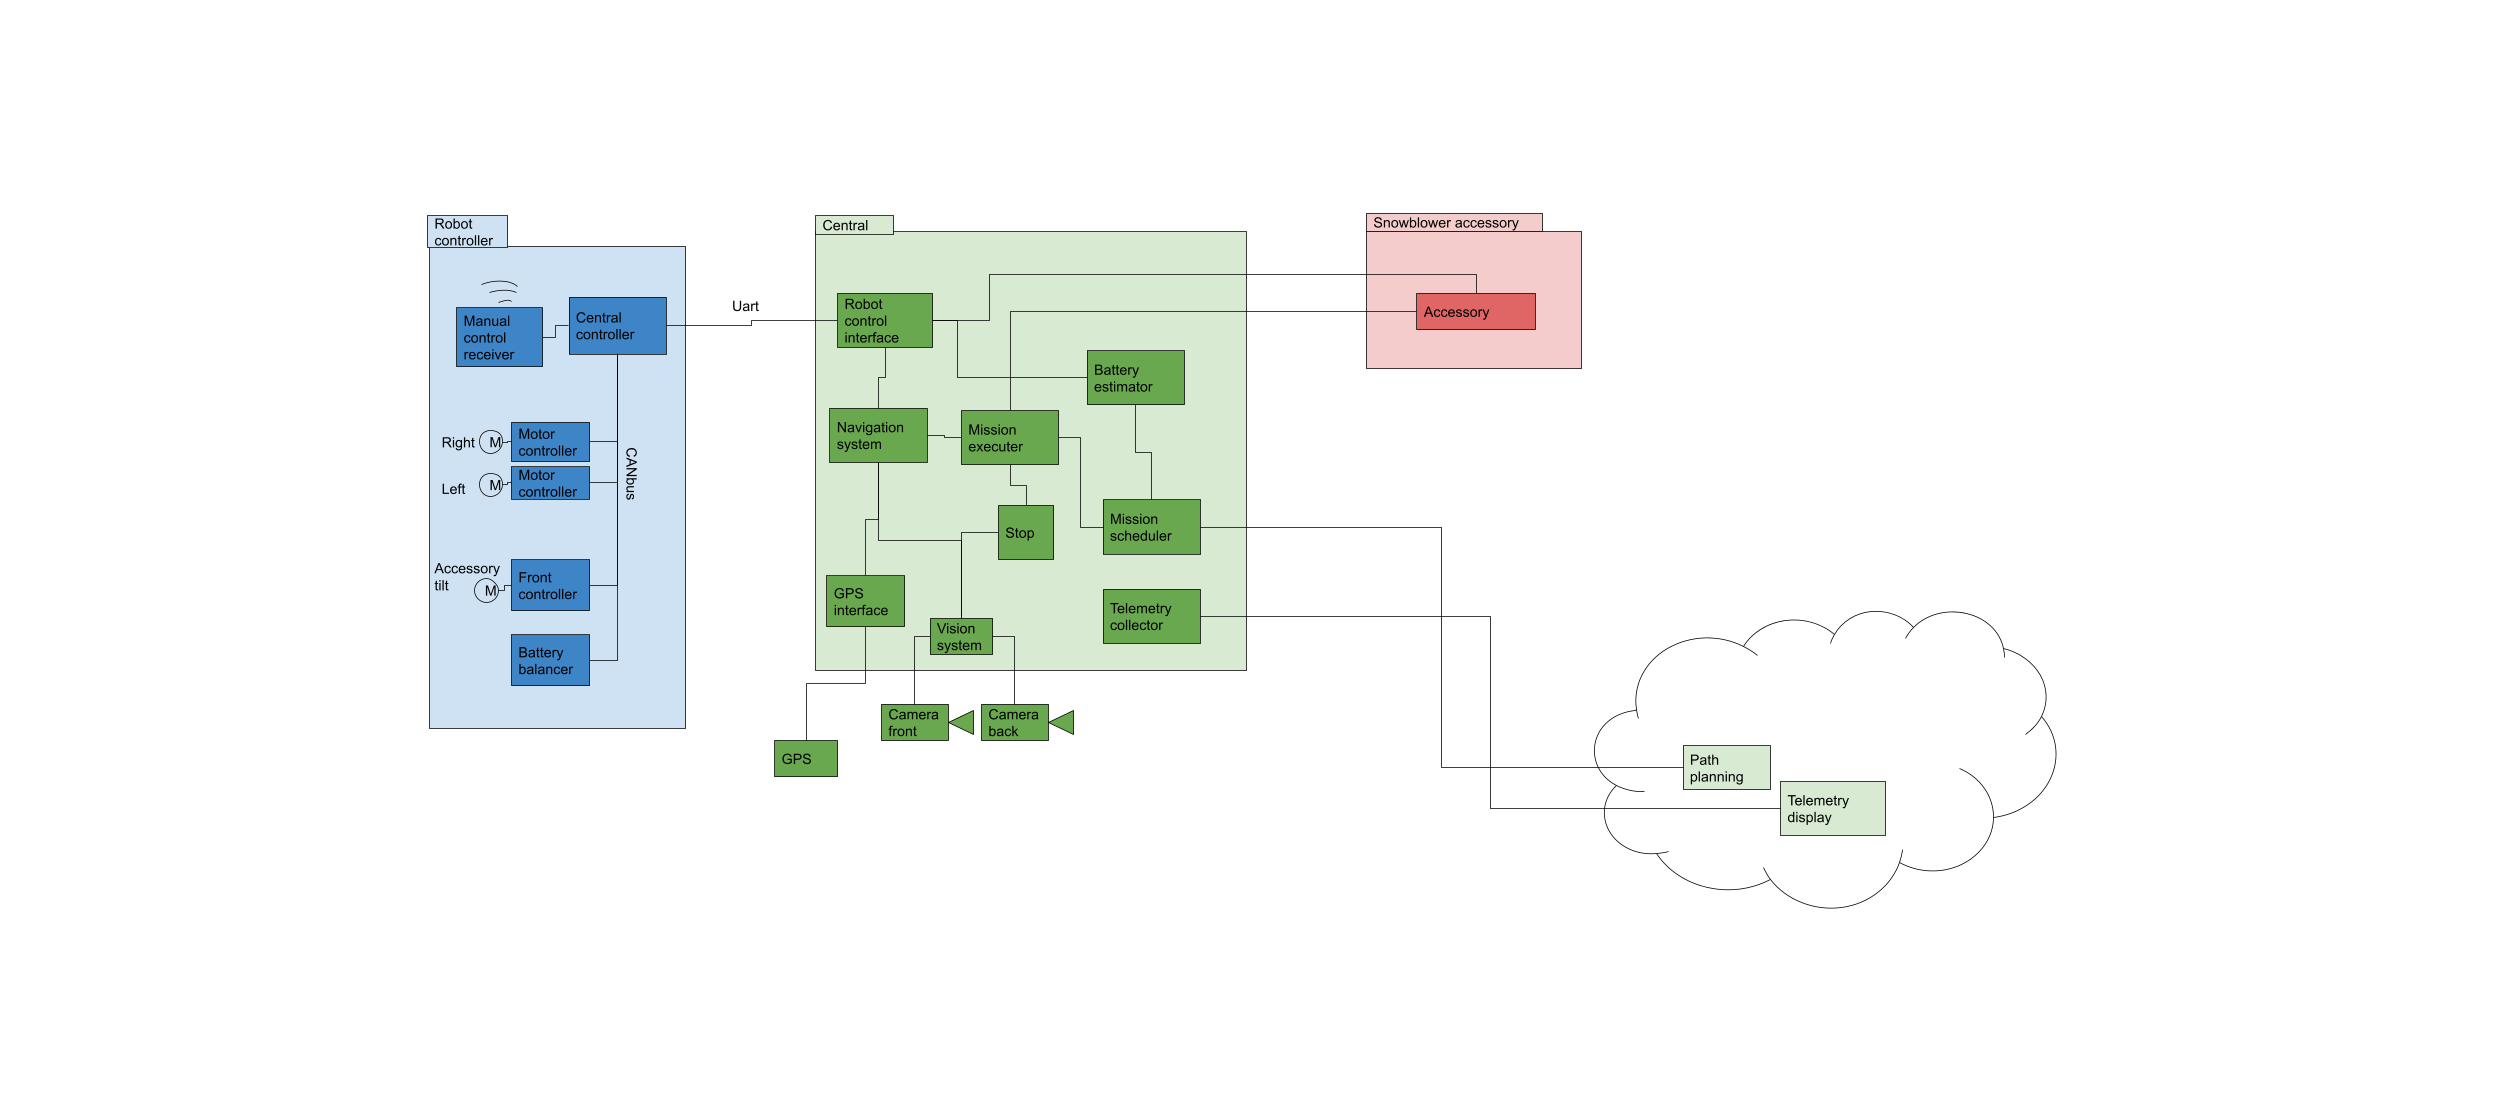
\includegraphics[width=\textwidth]{software_overview.png}
    \caption{Overview of the software architecture.}
    \label{fig:software_overview}
\end{figure}

The design of the software system is made up of different parts and are shown in figure \ref{fig:software_overview}. 
In figure \ref{fig:software_overview} each system is symbolized by a square with a describing name and
lines symbolize communication between systems. Some communication lines are omitted for clarity.

The design was divided into 4 main parts, each part has its own color in figure \ref{fig:software_overview}:

The safety critical part is shown in blue and controls the robot directly. This part is described in section (? ref to other Eriks part ?). The part communicate with the rest of the system over a UART \cite{IEEEUART} link with the Robot control interface system.

The non safety critical part is shown in the green big rectangle.
This part handles everything needed to do to carry out a mission and sends the proper commands to either the robot controller or the accessory.

The red part is the accessory, it controls the accessory directly.
The accessory is designed to be able to be any kind of accessory. In our test case it is a snowblower.

The last part in light green in the little cloud is running on a server somewhere. It is designed to be the interface between the robot and the world being able to get telemetry from the robot and send missions for it to do.

The green and red parts systems are arrowhead framework systems \cite{delsing2017arrowhead} running in a local cloud on the robot. By using the arrowhead framework these systems must each communicate with each other true well defined application programming interfaces (API). With these APIs a system can easily be changed out with another system implementing the same API or even more then one system implementing each implementing a part of the API.
The arrowhead framework also provides late binding between systems, witch means that a system only need to know the address of a service it needs to use when it actually want to use it at runtime.
To facilitate this late binding each arrowhead local cloud needs to have a set of core systems \cite{varga2017making}.

The systems in the cloud down to the right in figure \ref{fig:software_overview} is run in a separate arrowhead local cloud with it's own set of core systems. To be able to communicate with the other local cloud the gateway optional core system \cite{varga2015service} was used.

\subfile{figures/arrowhead_system_sequence2.tex}

To show how the systems may work together a sequence diagram is shown in figure \ref{fig:sequence2}.
In the sequence diagram the robot first do a mission where it navigates to a point and is preempted by a higher priority mission to charge the robot.
The way preemption is handled is that the mission executor when it's get a new mission will construct a new mission that will carry out the work left on the current mission and send this new mission to the mission scheduler.

\section{Result}
\label{sec:software:result}

To validate the design described in section \ref{sec:software:design} it was implemented.
The arrowhead systems where implemented in Java using a arrowhead application library \cite{arrowheadlib}.
For the core system of the arrowhead local cloud core-java-spring \cite{arrowheadcore} was used.
Due to time limitations was not the entire design implemented and only the local cloud on the robot was set up.
Table (? table ref ?) shows the status of completeness for each system implementation.

\section{Discussion}
How did the software design and implementation meet the design goals?

\section{Conclusion}
What was archived?
Further improvements?
hej

\printbibliography

\appendix
\section{Documentation}


\end{document}